%!TEX root = ../../common/main.tex

\chapter{Flavour Tagging}
\label{ch:flavour_tagging}

The time-dependent measurement of the $\CP$ asymmetry $\CPAsymmetry$ in the
decay of $\Bd$ and $\Bdbar$ mesons into the $\CP$ eigenstate $\Jpsi\KS$ requires
the knowledge of the \Bmeson flavour at production, \ie weather it contained
a $\bquark$ or a $\bquarkbar$. The method and algorithms used to infer this
information from all available event properties are named \enquote{flavour
tagging}.

Each tagging algorithm provides a tag $\tagdecision$ and a probability estimate
$\mistagestimate$ that the assigned tag is wrong, also called \enquote{mistag}
estimate. The tag is $\tagdecision=+1$ for an initial $\Bd$, $\tagdecision=-1$
for an initial $\Bdbar$, and $\tagdecision=0$ if the tagging algorithms were not
able to determine a decision. The mistag estimate interval is given by
$[0,0.5[$, where mistags $\mistagestimate^{\prime}>0.5$ are evaluated as
$\mistagestimate = 1 - \mistagestimate^{\prime}$ and the corresponding tag's
sign is reversed. If the algorithm is not able to determine a decision, the
mistag is set $\mistagestimate=0.5$.

The performance of the flavour tagging algorithms can be assigned using control
samples of \Bmesons whose final state determines the $\B$ flavour at decay
time (\ie are \enquote{flavour-specific}), \eg $\BuToJpsiK$ where the charge of
the kaon allows to infer the charge of the $\B$.

Given the numbers of all right tagged $\B$ candidates $\NRtagged$, all wrong
tagged candidates $\NWtagged$, and all \enquote{untagged} candidates
$\NUtagged$, the \enquote{tagging efficiency} $\tageff$ can be assigned
%
\begin{equation}\label{eq:flavour_tagging:tageff}
  \tageff = \frac{\NRtagged + \NWtagged}{\NRtagged + \NWtagged + \NUtagged}\eqpd
\end{equation}
%
In addition to the mistag estimate, the true underlying fraction of wrong tagged
candidates $\mistag$ is given by
%
\begin{equation}\label{eq:flavour_tagging:mistag}
  \mistag = \frac{\NWtagged}{\NRtagged + \NWtagged}\eqpd
\end{equation}
%
The statistically relevant \acl{FoM} for time-dependent measurements of $\CP$
violation\addref{for $\efftageff$ for CPV measurements}, the \enquote{effective
tagging efficiency}
%
\begin{equation}\label{eq:flavour_tagging:efftageff}
  \efftageff = \tageff(1 - 2 \mistag)^2 = \tageff \tagdilution^2 \eqcm
\end{equation}
%
represents the fraction of candidates necessary to reach the same statistical
power if the tagging would be perfect, and hence should be maximized to achieve
the best performance. The quantity $\tagdilution$ is called \enquote{dilution},
taking a value of $1$ in case of perfect tagging, and $0$ in case of random
tagging. As described in \cref{missing} the dilution can be directly translated
to the amplitude of the measured $\CP$ asymmetry. \missing{Effect of dilution on CPV asymmetry}

In the following sections more details of the flavour tagging are provided. A
short introduction of the utilized algorithms and a comparison to the flavour
tagging used at lepton colliders is given in \cref{sec:flavour_tagging:lhcb}.
\Cref{sec:flavour_tagging:os,sec:flavour_tagging:ss} describe the two different
classes of flavour tagging algorithms used at \LHCb, while the calibration of
the tagging algorithms outputs is described in
\cref{sec:flavour_tagging:calibration}. The combination of different algorithm
responses into a single decision is outlined in
\cref{sec:flavour_tagging:combination}. Performance numbers are provided in
\cref{sec:flavour_tagging:performance}, recent developments are discussed in
\cref{sec:flavour_tagging:developments}, and finally the experimental impact of
the flavour tagging on the measurement of $\CP$ violation in $\BdToJpsiKS$
decays is provided in \cref{sec:flavour_tagging:sin2beta}.

More details on the flavour tagging used by \LHCb can be found in
\cite{Aaij:2012mu}.

\section{Flavour tagging algorithms}
\label{sec:flavour_tagging:lhcb}

Several tagging algorithms, each specialized on different characteristics of the
underlying event, are used in order to determine the \Bmeson flavour at
production. The algorithms can be classified into two types: the \SS tagging and
\OS tagging algorithms, also called \SS/\OS taggers. The \SS taggers infer the
production flavour of the signal \Bmeson by identifying charged candidates
that have a high chance of being remnants of its hadronisation process. On the
other hand, the \OS taggers exploit the dominant production of \Bmesons
through $\bbbar$ quark pair production, allowing to partially reconstruct the
\bhadron produced together with each reconstructed signal \Bmeson and
thereby infer its initial flavour. \Cref{fig:flavour_tagging:lhcb:schematics}
gives an overview of the tagging algorithms used on the \acl{OS} and \acl{SS}.

The tagging algorithms are developed and trained using simulated $\BuToJpsiK$
and $\BdToDstarmunu$ decays. In an iterative procedure the selection criteria
were optimized in order to maximise the effective tagging efficiency
$\efftageff$. The algorithms only consider charged tracks with a good quality
of the track fit and momenta above $\SI{2}{\GeVc}$. Tracks with a polar angle of
less than $\SI{12}{\mrad}$ with respect to the beamline are declined. Further
on, particles originating from the signal candidate are suppressed by rejecting
all tracks that lie inside a cone of $\SI{5}{\mrad}$ around any signal $\B$
meson daughter. Using \IP requirements tracks from other \acp{PV} are
eliminated.

\Cref{sec:flavour_tagging:os,sec:flavour_tagging:ss} contain detailed
description of the \OS and \SS tagging algorithms. Recent developments that
exceed the scope of the analysis presented in this thesis but will be relevant
in the future are discussed in \cref{sec:flavour_tagging:developments}. Before
coming to the detailed description of the \LHCb flavour tagging algorithms, a
summary of the flavour tagging methods developed at \Babar and \Belle is given.

\begin{figure}
\centering
%!TEX root = ../../../common/main.tex

% Colours 
\definecolor{fcdOrnA}{HTML}{331605}
\definecolor{fcdOrnB}{HTML}{662C0A}
\definecolor{fcdOrnC}{HTML}{99420F}
\definecolor{fcdOrnD}{HTML}{CC5814}
\definecolor{fcdOrnE}{HTML}{FF6E19}
\definecolor{fcdOrnF}{HTML}{FF975B}
\definecolor{fcdOrnG}{HTML}{FFAC7C}
\definecolor{fcdOrnH}{HTML}{FFC19C}
\definecolor{fcdOrnI}{HTML}{FFD6BD}
\definecolor{fcdOrnJ}{HTML}{FFEADE}
\definecolor{fcdBluA}{HTML}{052A33}
\definecolor{fcdBluB}{HTML}{0A5466}
\definecolor{fcdBluC}{HTML}{0F7E99}
\definecolor{fcdBluD}{HTML}{14A8CC}
\definecolor{fcdBluE}{HTML}{19D2FF}
\definecolor{fcdBluF}{HTML}{5BDFFF}
\definecolor{fcdBluG}{HTML}{7CE5FF}
\definecolor{fcdBluH}{HTML}{9CECFF}
\definecolor{fcdBluI}{HTML}{9CECFF}
\definecolor{fcdBluJ}{HTML}{DEF9FF}
\definecolor{fcdGrnA}{HTML}{243304}
\definecolor{fcdGrnB}{HTML}{476608}
\definecolor{fcdGrnC}{HTML}{6B990D}
\definecolor{fcdGrnD}{HTML}{A0E02D}
\definecolor{fcdGrnE}{HTML}{B2FF15}
\definecolor{fcdGrnF}{HTML}{C8FF58}
\definecolor{fcdGrnG}{HTML}{D3FF79}
\definecolor{fcdGrnH}{HTML}{DEFF9B}
\definecolor{fcdGrnI}{HTML}{E9FFBC}
\definecolor{fcdGrnJ}{HTML}{F4FFDE}
\definecolor{fcdVltA}{HTML}{310433}
\definecolor{fcdVltB}{HTML}{620866}
\definecolor{fcdVltC}{HTML}{930D99}
\definecolor{fcdVltD}{HTML}{C411CC}
\definecolor{fcdVltE}{HTML}{F514FF}
\definecolor{fcdVltF}{HTML}{F858FF}
\definecolor{fcdVltG}{HTML}{F979FF}
\definecolor{fcdVltH}{HTML}{FB9BFF}
\definecolor{fcdVltI}{HTML}{FCBCFF}
\definecolor{fcdVltJ}{HTML}{FEDDFF}

\definecolor{fcdGrayA}{HTML}{111111}
\definecolor{fcdGrayB}{HTML}{222222}
\definecolor{fcdGrayC}{HTML}{333333}
\definecolor{fcdGrayD}{HTML}{444444}
\definecolor{fcdGrayE}{HTML}{555555}
\definecolor{fcdGrayF}{HTML}{666666}
\definecolor{fcdGrayG}{HTML}{777777}
\definecolor{fcdGrayH}{HTML}{888888}
\definecolor{fcdGrayI}{HTML}{999999}
\definecolor{fcdGrayJ}{HTML}{AAAAAA}
\definecolor{fcdGrayK}{HTML}{BBBBBB}
\definecolor{fcdGrayL}{HTML}{CCCCCC}
\definecolor{fcdGrayM}{HTML}{DDDDDD}
\definecolor{fcdGrayN}{HTML}{EEEEEE}

\definecolor{fcdTropiteal}    {HTML}{00A8C6}
\definecolor{fcdTealDrop}     {HTML}{40C0CB}
\definecolor{fcdWhiteTrash}   {HTML}{F9F2E7}
\definecolor{fcdAtomicBikini} {HTML}{AEE239}
\definecolor{fcdFeebleWeek}   {HTML}{8FBE00}





\colorlet{ClrTxt}{black}
\colorlet{ClrTxtVeryDarkGray}{fcdGrayE}
\colorlet{ClrTxtDarkGray}{fcdGrayJ}
\colorlet{ClrVtxGray}{fcdGrayM}

\colorlet{ClrSigQuark}{fcdTealDrop}
\colorlet{ClrSigMeson}{fcdTropiteal}
\colorlet{ClrSigArrow}{fcdTropiteal}

\colorlet{ClrTagQuark}{fcdAtomicBikini}
\colorlet{ClrTagMeson}{fcdFeebleWeek}
\colorlet{ClrTagArrow}{fcdFeebleWeek}

\begin{tikzpicture}[
  scale=1, 
  >=stealth',
  font=\small,
  quark_sig/.style={
    align=center, 
    minimum size=3ex,
    circle,
    color=ClrSigQuark,
    fill=ClrSigQuark,
    text=ClrTxt,
    draw, 
    thick,
    inner sep=0pt,
    outer sep=0pt,
    node distance=0ex
  },
  quark_tag/.style={
    align=center, 
    minimum size=3ex,
    circle,
    color=ClrTagQuark,
    fill=ClrTagQuark,
    text=ClrTxt,
    draw, 
    thick,
    inner sep=0pt,
    outer sep=0pt,
    node distance=0ex
  },
  meson_sig/.style={
    draw, 
    align=center, 
    minimum size=4.5ex,
    circle,
    color=ClrSigMeson,
    fill=ClrSigMeson,
    text=ClrTxt,
    thick,
    inner sep=0pt,
    outer sep=1pt,
    node distance=0ex
  },
  meson_tag/.style={
    draw, 
    align=center, 
    minimum size=4.5ex,
    circle,
    color=ClrTagMeson,
    fill=ClrTagMeson,
    text=ClrTxt,
    thick,
    inner sep=0pt,
    outer sep=1pt,
    node distance=0ex
  },
  meson_comb/.style={
    shape=ellipse, 
    draw,
    fill,
    very thick,
    inner sep=0pt,
    outer sep=0pt,
    minimum width=8ex,
    minimum height=5ex},
  vertex/.style={
    shape=ellipse,
    draw,
    inner sep=1ex,
    outer sep=0pt,
    minimum width=10ex,
    minimum height=10ex,
    color=ClrVtxGray,
    fill=ClrVtxGray,
    text=ClrTxt,
    node distance=1ex
  },
  vertex_label/.style={
    inner sep=0pt,
    outer sep=0pt,
    text=ClrTxtDarkGray,
    node distance=1ex,
    font=\sffamily\small
  },
  tagger_label/.style={
    inner sep=0pt,
    outer sep=0pt,
    text=ClrTxtVeryDarkGray,
    node distance=1ex,
    font=\sffamily\small    
  },
  arrow_sig/.style={
    ->,
    very thick,
    color=ClrSigArrow
  },
  arrow_tag/.style={
    ->,
    very thick,
    color=ClrTagArrow
  }
]

%\draw[help lines] (-1,-5) grid (11,5);

\draw[dashed,color=fcdGrayE] (0,0) -- (12,0);
\node[text width=2.5cm,text=ClrTxtDarkGray,font=\sffamily\small] (SST) at (10.5,+0.3) {\hfill same side};
\node[text width=2.5cm,text=ClrTxtDarkGray,font=\sffamily\small] (OST) at (10.5,-0.3) {\hfill opposite side};


\node[draw,circle,fill,color=ClrSigQuark,inner sep=0pt,minimum size=8pt] 
  (coll) at (0,0) {};

\draw[<-,very thick] (coll) -- (+1,0);
\draw[->,very thick] (-1,0) -- (coll);

\begin{pgfonlayer}{foreground}
  
  % bbbar
  \node[quark_sig] (qrk_bbar) at (0.2,+0.8) {$\bquarkbar$};
  \node[quark_sig] (qrk_b) at (0.2,-0.8) {$\bquark$};
  
  \path (qrk_bbar) 
        to[circle connection bar switch color=from (ClrSigQuark) to (ClrSigQuark)] 
        (coll);
  \path (qrk_b) 
        to[circle connection bar switch color=from (ClrSigQuark) to (ClrSigQuark)] 
        (coll);
  
  % Signal decay
  \node[meson_sig,color=ClrSigMeson,fill=ClrSigMeson,text=ClrTxt] (SigJpsi) at (7.5,+2.25) {$\Jpsi$}  ;
  \node[meson_sig,color=ClrSigMeson,fill=ClrSigMeson,text=ClrTxt] (SigKS) [below=of SigJpsi] {$\KS$}  ;
  
  % SS tagging
  \path (qrk_bbar) ++(15:3ex) node (qrk_d) [quark_tag] {$\dquark$};
  
  \node[quark_tag] (qrk_dbar) at (0.8,+2.2) {$\dquarkbar$};
  
  \node[draw,circle,fill,color=ClrTagQuark,inner sep=0pt,minimum size=4pt] 
    (vacuumexc) at ([xshift=-2ex] $(qrk_dbar)!0.5!(qrk_d)$) {};
  
  \path (qrk_d) 
        to[circle connection bar switch color=from (ClrTagQuark) to (ClrTagQuark)] 
        (vacuumexc);
  \path (qrk_dbar) 
        to[circle connection bar switch color=from (ClrTagQuark) to (ClrTagQuark)] 
        (vacuumexc);  
  \path (qrk_dbar) ++(165:3ex) node (qrk_u)    [quark_tag] {$\uquark$};

  \node[meson_tag] (SSpip) at (3.3,+2.7) {$\pip$}; 
  

  % OS tagging
  \path (qrk_b)    ++(-15:3ex) node (qrk_xbar) [quark_tag] {$\quarkbar$};  

  % Tagging particles 
  \node[meson_tag] (OSlepton) at (9.5,-2.25) {$\lepm$};
  \node[meson_tag] (OSkaon)   at (9.5,-1)    {$\Kp$};
  
\end{pgfonlayer} 
  
  
\node[meson_comb,rotate=+15,color=ClrSigMeson,text=ClrTxt] (SigBz) at ($(qrk_bbar)!0.5!(qrk_d)$) {  }; 
\node[meson_comb,rotate=-15,color=ClrTagMeson,text=ClrTxt] (Hb) at ($(qrk_b)!0.5!(qrk_xbar)$) {}; 
\node[meson_comb,rotate=-15,color=ClrTagMeson,text=ClrTxt] (pip_SS) at ($(qrk_dbar)!0.5!(qrk_u)$)   {}; 

  
\begin{pgfonlayer}{background}
  \node[vertex,fit=(SigBz)(Hb)(pip_SS),minimum width=16ex] (PV) {};
  \node[vertex_label,align=center] (PV_label) [above=of PV] {PV};
  
  \node[vertex,fit=(SigJpsi)(SigKS)   ,minimum width=10ex] (SigSV) {};
  \node[vertex_label,align=center] (SigSV_label) [above=of SigSV] {SV};
  
  \node[vertex,minimum width=11ex,minimum height=9ex,align=left] (OS_SV) at (4.5,-1.75) {$\bquark \to \cquark$\\  $\bquark \to X \lepm$};
  \node[vertex_label,align=center] (OS_SV_label) [above=of OS_SV] {SV};
  
  
  \node[vertex,minimum width=9ex,minimum height=7ex,align=center] (OS_TV) at (7.5,-1.25) {$\cquark \to \squark$};
\end{pgfonlayer}


\begin{pgfonlayer}{foreground}
  \draw[arrow_sig] (SigBz)  -- node (Bz_label) [above] {$\Bd$} ([xshift=+4pt] SigSV.west);
  \draw[arrow_sig] let \p1 =(SigJpsi.east) in (\x1-1,\y1+2)  -- (\x1+50,\y1+5);
  \draw[arrow_sig] let \p1 =(SigJpsi.east) in (\x1-1,\y1-2)  -- (\x1+50,\y1-5);
  \draw[arrow_sig] let \p1 =(SigKS.east)   in (\x1-1,\y1+2)  -- (\x1+50,\y1+5);
  \draw[arrow_sig] let \p1 =(SigKS.east)   in (\x1-1,\y1-2)  -- (\x1+50,\y1-5);
    
  \draw[arrow_tag] (Hb)     -- node (Hb_label) [above] {$\hb$}  ([xshift=+4pt] OS_SV.west);
  \draw[arrow_tag] (OS_SV)  -- ([xshift=+4pt] OS_TV.west);
  \draw[arrow_tag] (OS_SV)  -- ([xshift=+0pt] OSlepton.west);
  \draw[arrow_tag] (OS_TV)  -- ([xshift=+0pt] OSkaon.west);
  \draw[arrow_tag] (pip_SS) -- ([xshift=+0pt] SSpip.west);


  \node[tagger_label,align=left] (SSpip_label) [right=of SSpip] {SS pion};
  \node[tagger_label,align=left] (OSlepton_label) [right=of OSlepton] {OS muon\\ OS electron};
  \node[tagger_label,align=left] (OSkaon_label)   [right=of OSkaon] {OS kaon};
  \node[tagger_label,align=center] (OSVtcCh_label) [below=of OS_SV] {OS vertex charge};

\end{pgfonlayer}

\end{tikzpicture}

\caption{Schematic overview of the used \acs*{OS} and \acs*{SS} tagging
algorithms. \cite{wishahi:2013jt}}
\label{fig:flavour_tagging:lhcb:schematics}
\end{figure}

\subsection*{Flavour tagging at \Babar and \Belle}
\label{sec:flavour_tagging:lhcb:b_factories}
Caused by the different nature of the experimental setup the tagging method used
at \LHCb differs from methods used at the \BFactories. As described in
\cref{sec:lhcb_experiment:detector} the \bhadron production is dominated
by gluon-gluon fusion over a large range of $q^2$ in contrast to the production
at the $\YFourS$ $\bbbar$ resonance as it is the case at the \BFactories. The
following section gives a résumé of the flavour tagging methods employed by the
\Babar and \Belle collaborations outlined in \Ref~\cite[][Ch. 8]{Bevan:2014iga}.
%
\begin{figure}
\centering
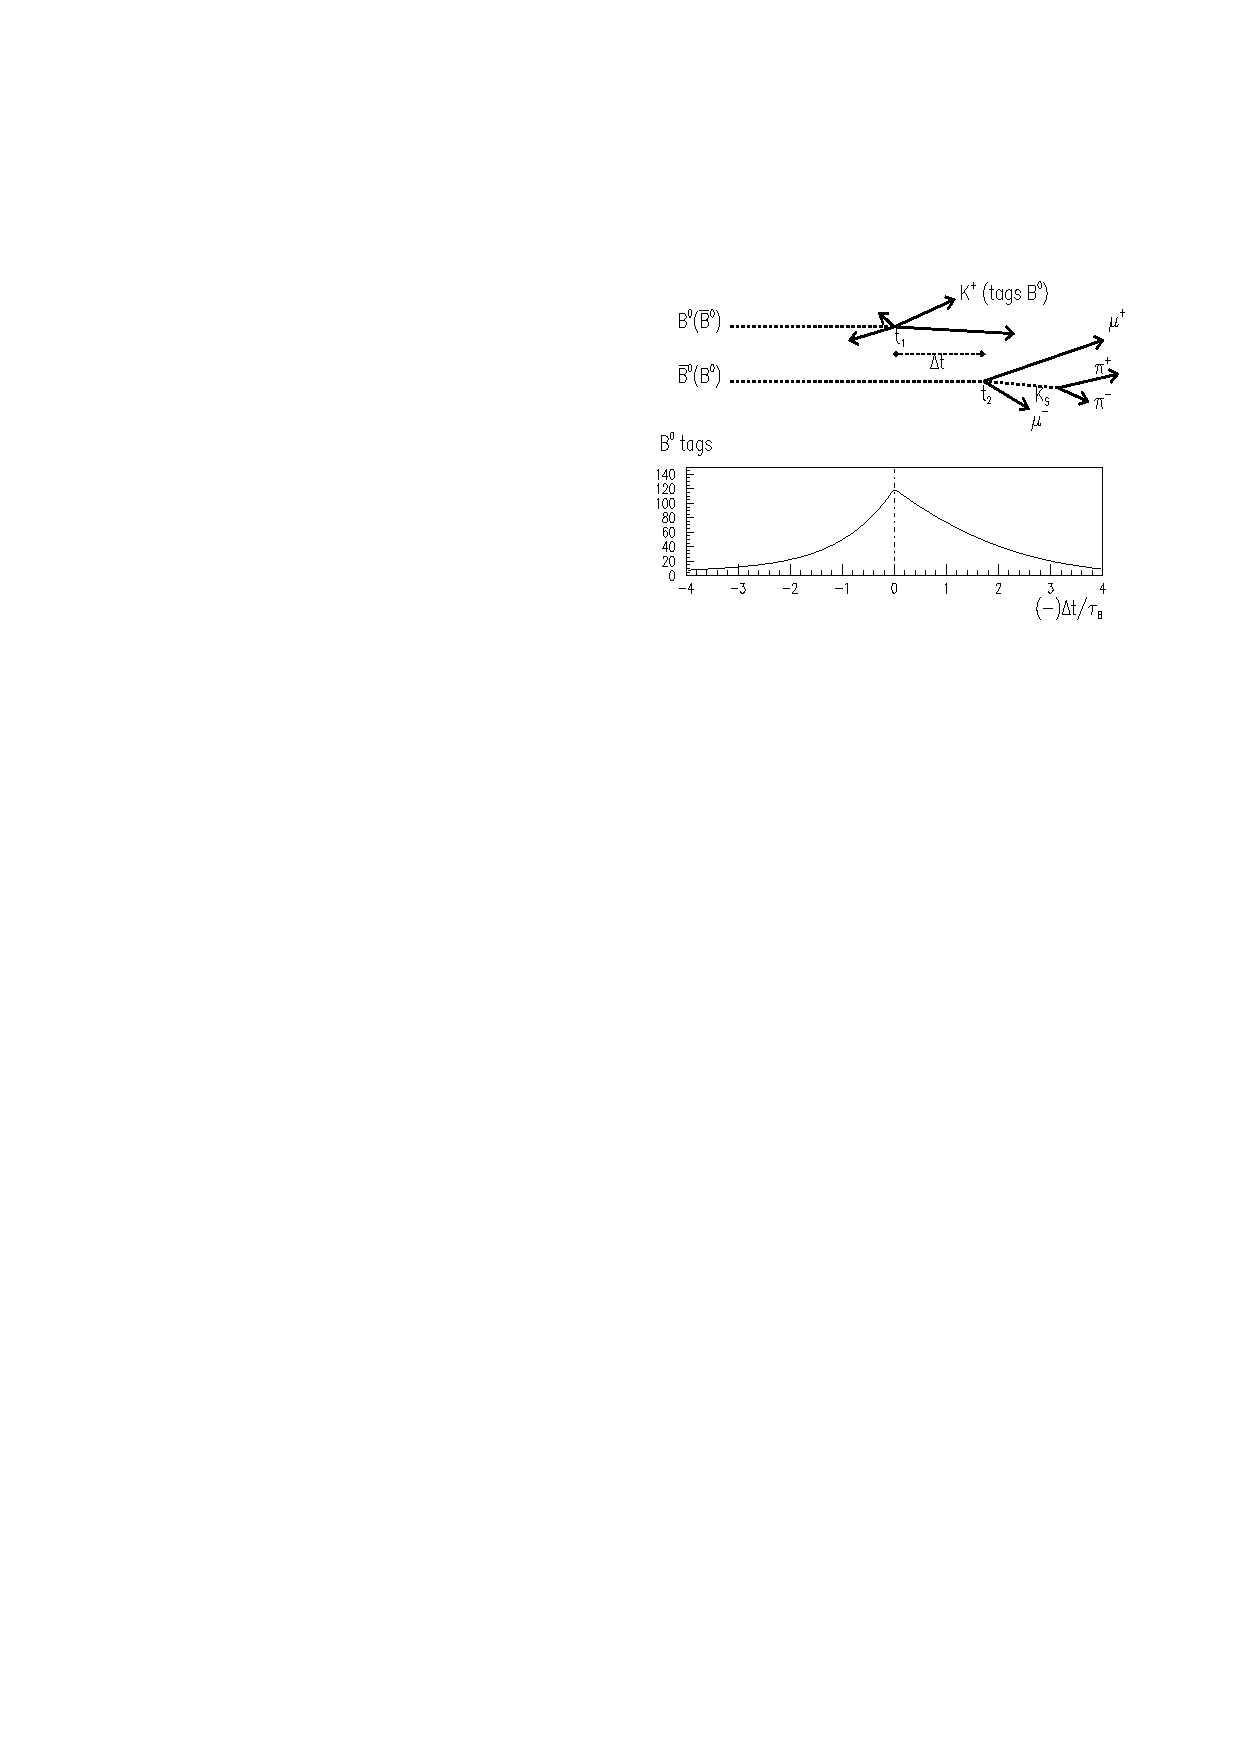
\includegraphics[width=\textwidth]{private/content/flavour-tagging/figs/b_factory_basic_principles}
\caption{Illustration of the measurement of \sintwobeta as conducted by the
\BFactories. \cite{Bevan:2014iga}}
\label{fig:flavour_tagging:lhcb:b_factory_basic_principles}
\end{figure}

\Cref{fig:flavour_tagging:lhcb:b_factory_basic_principles} illustrates the basic
principles of a \CP violation measurement at the \BFactories. The produced
$\Bd\Bdbar$ pair's wave function is in a $P$-wave entangled state, until one of
the mesons decays. From this point in space time ($t_1$) the second $\B$ meson
propagates further through the detector, mixes to its antimatter state, and
finally decays at $t_2$. The \CP asymmetry $\CPAsymmetry$ will therefore be a
function of the decay time difference $\Delta t$. This has two implications:
First, the decay time difference will always be computed relative to the
\enquote{tagging} \Bmeson decay and thus might be negative if the signal $\B$
meson decays first. Secondly, if the tagging \Bmeson decays into a
flavour-specific final state, this specifies the signal \Bmeson's flavour at
$\Delta t=0$.

As a result of the production mechanism, the fully reconstructed signal decay
leaves all remaining tracks to originate from the tagging $\B$. This allows to
classify the decay of the tagging meson according to the signature of the final
state particles. Specialised taggers then identify decays based on their
specific signature. In a second stage, all results provided by the single
taggers are combined into a final tagging decision. 

The lepton taggers deduce a tag from the charge of electrons and muons from
$\bquark \to \cquark \lepm \neutrinobar$ transitions in semileptonic $\B$
decays. Likewise, second order transitions from $\bquark \to \Wm \cquark ( \to
\squark \lepp \neutrino )$ can be used, but has to be handled differently as
their charge is opposite compared to primary leptons. Charged kaon candidates
from the $\bquark \to \cquark \to \squark$ decay chain reflect the charge of the
tagging meson. Here as well, kaons from second order transitions carry the
opposite charge. Charged pions from charm decays work as tagging particles
either directly or in events with both a pion and a charged kaon, the
correlation of the particles can be utilised to improve the tag decision.
Selecting high momentum particles, \eg fast pions from $\Bdbar \to \Dstarp
\pim$, is on its own another source of tagging information and might
additionally be correlated with slow particles to enhance the tagging result.
Finally the flavour of $\Lambda$ baryons from decays of the tagging $\B$ meson
can be exploited.

The \Babar experiment uses \acp{ANN} for each single tagger to provide several
intermediate tagging decisions that are subsequently combined using another \ANN
to gain a joined tagging decision. The effective tagging efficiency of the final
\Babar tagging algorithm is estimated on data to be $\efftageff = \SI{33.1 +-
0.3}{\percent}$. In \Belle analyses the flavour tagging approach is similar.
Instead of \acp{ANN} multi-dimensional look-up tables are used. At first,
information from charged tracks are looked-up to sort them into the signature
categories. Next, the received results are used on an event-level to provide the
final tagging decision. Using this approach an effective tagging efficiency of
$\efftageff = \SI{30.1 +- 0.4}{\percent}$ is achieved.

\subsection{\Acl{OS} algorithms}
\label{sec:flavour_tagging:os}
The \OS algorithms all infer the tagging decision from the quark flavour of the
\bhadron produced in association with the signal \Bmeson. If for example a $\Bu$
decays into a $\Kp X$ final state trough $\bquarkbar \to \cquarkbar \to
\squarkbar$ transition, it can unambiguously stated by looking at the kaon
charge that the \bhadron produced along with the $\Bu$ contained a $\bquarkbar$
quark. The tag identification for events with this signature fall into the scope
of the \OSK tagger.

In total four distinct \OS taggers, each developed for a special \OS decay
signature, provide tagging information. Besides the \OSK tagger, the \OSe and
the \OSm select leptons coming from the primary $\bquark \to X \lepm$ decay to
use their charge as an information carrier of the $\B$ flavour. Finally, the
\OSvtx tagger performs an inclusive reconstruction of the \OS \SV to then
compute a weighted sum of all particle track charges that originate from the
\SV. In the following the selection criteria and algorithms of the \OS taggers
are briefly described.

\missing{Intrinsic mistag due to neutral B meson oscillation}
 
\subsubsection{The \acl{OSK} tagger}
\label{sec:flavour_tagging:os:kaon}
The kaon tagger exploits the charge of kaons stemming from $\bquark \to
\cquark \to \squark$ decays of the opposite side \bhadron. As the charge of the
kaon is the opposite of the ancestor's charge, the kaon always carries the same
charge as the signal \Bmeson.

To reduce background contributions of prompt kaons and kaons from primary
$\bquarkbar \to \Wm (\to \cquark \squarkbar) \cquarkbar$ transitions, in which
case the kaon carries the \enquote{wrong} charge, several selection criteria are
applied. Cuts on the \pT, the \IP, the \IP/$\sigma_\text{\IP}$, and the track
fit \chisqndf are performed. \PID requirements on the \DLLKpi, the \DLLppi, and
\DLLmupi suppress mis-identified particles. Clone tracks are removed and kaon
candidates with originate from other \acp{PV} are rejected using a cut on the
\IP/$\sigma_\text{\IP}$ with respect to any \PV.
\cref{tab:flavour_tagging:os:kaon:cuts} lists all applied cuts. If more than one
tagging candidate is found, the decision obtained from the candidate with the
highest \pT is chosen. To further increase the effective tagging efficiency only
tag decisions are considered if the estimated mistag probability is smaller than
$\mathcal{P}=0.46$.

\begin{table}
  \centering
  \caption{Selection cuts for the \OSK tagger \cite{Grabalosa:2012qra}.}
  \label{tab:flavour_tagging:os:kaon:cuts}
  \begin{tabular}{ll}
    \toprule
    Property & Value \\
    \midrule
    \pT                                       & $>\SI{0.5}{\GeVc}$                  \\
    \IP                                       & $<\SI{1.25}{\milli\metre}$          \\
    \IP$/\sigma_\text{\IP}$                   & $>\num{3.35}$                       \\
    track fit \chisqndf                       & $<\num{2.75}$                       \\
    \DLLKpi                                   & $>\num{6}$                          \\
    $(\DLLKpi - \DLLppi)$                     & $>\num{-4}$                         \\
    \IP$/\sigma_\text{\IP}$ \wrt any \PV      & $>\num{4.5}$                        \\
    reject clone tracks & \\
    \bottomrule
  \end{tabular}
\end{table}

\subsubsection{The \acl{OSe} and the \acl{OSm} taggers}
\label{sec:flavour_tagging:os:lepton}

Leptons from $\bquark \to \cquark\Wboson$ transitions are selected in order to
deduce the opposite \bhadron charge. Thus positive lepton charge indicates a
$\bquark$ quark content of the signal \Bmeson and vice versa.

Cuts on the \PID and the lepton \pT are applied to reduce the mis-identification
rate and to suppress leptons from secondary decays of charm mesons. The muon
candidate purity is further enhanced by reducing fake muons, clone tracks, and
requiring a sufficient track fit quality. Electron candidate tracks must lie
inside the \HCAL acceptance and leave a substantial energy deposition in the
\ECAL compared to their momentum. To reduce backgrounds from photon conversions
close to the \proton\proton interaction region, a upper limit on the maximal
ionisation charge $Q_\text{\VELO}$ deposited in the \VELO is set. If more than
one lepton candidate passes the requirements, the one with the highest \pT is
chosen.

\begin{table}
  \centering
  \caption{Selection cuts for the \OSe and \OSm taggers
  \cite{Grabalosa:2012qra}, where $E$ is the particle energy measured in the
  \ac{ECAL} and $p$ the measured particle momentum. $Q_\text{\VELO}$ describes
  the ionisation charge deposit in the \VELO.}
  \label{tab:flavour_tagging:os:lepton:cuts}
  \begin{tabular}{ll}
    \toprule
    % general
    Property                                  & Value                               \\
    \midrule
    lepton \pT                                & $>\SI{1.2}{\GeVc}$                  \\
    muon \DLLmupi                             & $>\num{1}$                          \\
    muon track fit \chisqndf                  & $<\num{3.2}$                        \\
    \multicolumn{2}{l}{reject muon clone tracks and fake muons}                     \\
    electron \DLLepi                          & $>\num{4}$                          \\
    electron $E/p$                            & $>\num{0.8}$                        \\
    max. electron $Q_\text{\VELO}$            & $<\num{1.6}$                        \\
    \multicolumn{2}{l}{electron candidate track in \HCAL acceptance}                \\
    \bottomrule
  \end{tabular}
\end{table}

\subsubsection{The \acl{OSvtx} tagger}
\label{sec:flavour_tagging:os:vertex}

Besides the single particle taggers for kaons, muons, and electrons, the
\acl{OSvtx} tagger follows an alternative approach by trying to inclusively
reconstruct the decay vertex of the opposite \bhadron. Starting with a two-track
seed, matching tracks are appended and a weighted sum of the vertex charge is
calculated. The procedure is optimized using cuts on the considered tracks, the
seed properties, and the features of the reconstructed vertex.

The initial vertex seed is found by sampling track pairs from all particle
candidates surviving the following criteria: At least one of the tracks must be
a long track with a track fit quality of $\chisqndf<\num{2.5}$. To exclude poor
track reconstruction only tracks with an \IP uncertainty of
$\sigma_\text{\IP}<\num{1}$ are taken into account. Tracks from prompt particles
are rejected by a cut on the $2.5<\text{\IP}/\sigma_\text{\PV}<100$ \wrt the
\PV. Additionally the track has to have a $\pT>\SI{0.15}{\GeVc}$ and an
\IP$<\SI{3}{\milli\metre}$ \wrt to the \PV.\todo{Understand why the two IP
criteria are conflicting} The two seed tracks must be separated by an angle of
$\phi>\SI{1}{\mrad}$ and one of the tracks has to have a $\pT>\SI{0.3}{\GeVc}$.

For tracks pairs passing all selection criteria a vertex fit is performed. If
the fit succeeds and a fit quality of at least $\chisqndf<10$ is met, the fitted
vertex is considered as a seed. The seed is required to lie inside the detector
acceptance and in the forward direction of the \PV ($z>0$). \missing{Define
$r$-distance} The invariant mass of the seed is calculated and has to be greater
than $\SI{0.2}{\GeVcc}$ and not be compatible with the known $\KS$ or $\Lambdaz$
masses. % 0.490 < m_KS < 0.505 and 1.11 < m_Lambda < 1.12
A likelihood is computed for all seeds considering the vertex fit $\chisqndf$,
the minimum \pT, the maximum \PV \IP, the minimum \PV \IP$/\sigma_\text{\IP}$,
the angle between the seed tracks, the $r$-distance and the angle between the
seed direction \wrt to the \PV. Only seeds with a likelihood greater $\num{0.6}$
are further considered and the seed with the maximum likelihood is selected. The
seed algorithm successfully finds a seed in nearly $\SI{50}{\percent}$ of all
events and has a rate of $\SI{60}{\percent}$ to find a seed that is formed by
\bhadron decay products.

Subsequently more tracks are added to the seed. Additional tracks are required
to be compatible with the reconstructed seed vertex
(\IP$<\SI{0.9}{\milli\metre}$), have a \DOCA to any track in the seed smaller
than $\SI{0.2}{\milli\metre}$, the track fit quality is at least
$\chisqndf<\num{3}$, and are ruled out to be a clone track. Additionally the \IP
with respect to the \PV has to be larger than $\SI{0.1}{\milli\metre}$ and
$\text{\IP}/\sigma_\text{\IP}>\num{3.5}$.

After all tracks are added to the vertex another set of selection requirements
has to be fulfilled to optimize the effective tagging efficiency. The sum of all
track momenta has to be $\sum_i p_i > \SI{10}{\GeVc}$ and $\sum_i \pT(i) >
\SI{10}{\GeVc}$, the invariant vertex mass must be greater than $m_\text{vtx} >
\SI{0.5}{\GeVcc}$, the sum of the track
$\sum_i\text{\IP}_i/\sigma_{\text{\IP}_i}$ has to be larger $\num{10}$ and the
sum of the track \DOCA has to be $\sum_i\text{\acs{DOCA}}_i <
\SI{0.5}{\milli\metre}$.

The tag decision is then deduced from the inclusively reconstructed vertex by
calculating the weighted charge for all tracks $i$ forming the vertex
%
\begin{equation}\label{eq:flavour_tagging:os:vertex:charge}
  Q_\text{vtx} = \frac{\sum_i \pT^k(i)Q_i}{\sum_i\pT^k(i)}\eqcm
\end{equation}
where the track \acp{pT} are used as weights and the $k$ parameter is optimised
using simulated data to be $k=\num{0.4}$. In a final step, only charges of
$\vert Q_\text{vtx} \vert > 0.25$ are considered and the mistag probability has
to be smaller than $\mathcal{P}=0.46$.

\subsection{\Acl{SS} algorithms}
\label{sec:flavour_tagging:ss}

The \acl{SS} taggers exploit charge information from pions or kaons produced in
the hadronisation process of the signal \Bmeson. As illustrated in
\cref{fig:flavour_tagging:lhcb:schematics} the $\qqbar$ quark pair produced
alongside the signal meson, splits up to form the $\B$ meson and in the case of
a $\Bd$ ($\Bs$) an accompanying pion (kaon). Pions might also be produced in the
decay of excited $\B$ meson states.

\subsubsection{The \acl{SSpi} tagger}
\label{sec:flavour_tagging:ss:pion}

The pions from either the \Bmeson hadronisation or the decay of excited states
carry the same charge as the signal \Bmeson and are therefore suitable to
extract tagging information. The selection criteria pion candidates are required
to fulfil are listed in \cref{tab:flavour_tagging:ss:pion:cuts}. If more than
one pion candidate passes the requirements, the one with the highest \pT is
chosen. The tag decision has to have a mistag probability of $\mathcal{P}<0.46$,
otherwise the tag decision will be refused.
%
\begin{table}
  \centering
  \caption{Selection cuts for the \SSpi tagger \cite{Grabalosa:2012qra}, where
  $\Delta Q$ describes the mass difference of the $\Bd\pion$ mass and the $\Bd$
  mass.}
  \label{tab:flavour_tagging:ss:pion:cuts}
  \begin{tabular}{ll}
    \toprule
    Property                                  & Value                               \\
    \midrule
    \multicolumn{2}{l}{only long track pion candidates}                             \\
    \DLLKpi                                   & $<\num{4.5}$                        \\
    \DLLppi                                   & $<\num{15}$                         \\
    \pT                                       & $>\SI{0.5}{\GeVc}$                  \\
    $p$                                       & $>\SI{2.5}{\GeVc}$                  \\
    \PV $\text{\IP}/\sigma_\text{\IP}$        & $<\num{4}$                          \\
    $\Delta Q$                                & $<\SI{1.5}{\GeVcc}$                 \\
    \bottomrule
  \end{tabular}
\end{table}

\subsubsection{The \acl{SSK} tagger}
\label{sec:flavour_tagging:ss:kaon}

The charge of kaons produced together with a signal $\Bs$ meson can be exploited
in order to get a tag decision. \Cref{tab:flavour_tagging:ss:kaon:cuts} shows
all selection requirements for kaon candidates. If more than one candidate
passes the criteria, the one with the highest \pT is used. As this thesis
presents a measurement in the decay of $\Bd$ and $\Bdbar$ mesons, where the kaon
tagger is not used, no further details will be given and the emphasis is placed
on the \SSpi tagger.
%
\begin{table}
  \centering
  \caption{Selection cuts for the \SSK tagger \cite{Grabalosa:2012qra}, where
  $\Delta Q$ describes the mass difference of the $\Bs\kaon$ mass and the $\Bs$
  mass, $\vert \Delta\phi \vert$ the difference in the $\phi$ angle between the
  signal \Bmeson and the kaon, $\vert \Delta\eta \vert$ the pseudo-rapidity
  between the signal \Bmeson and the kaon, and $\vert \Delta R \vert =
  \sqrt{\Delta\eta^2 + \Delta\phi^2}$.}
  \label{tab:flavour_tagging:ss:kaon:cuts}
  \begin{tabular}{ll}
    \toprule
    Property                                  & Value                               \\
    \midrule
    \DLLKpi                                   & $>\num{4.5}$                        \\
    (\DLLKpi - \DLLppi)                       & $>\num{-8.5}$                       \\
    \pT                                       & $>\SI{0.75}{\GeVc}$                 \\
    $p$                                       & $>\SI{5.25}{\GeVc}$                 \\
    \PV $\text{\IP}/\sigma_\text{\IP}$        & $<\num{4.125}$                      \\
    track $\chisqndf$                         & $<\num{3.75}$                       \\
    $\Delta Q$                                & $<\SI{1.5}{\GeVcc}$                 \\
    $\vert \Delta\phi \vert$                  & $<\num{0.7}$                        \\
    $\vert \Delta\eta \vert$                  & $<\num{0.525}$                      \\
    $\vert \Delta R \vert$                    & $<\num{1.2}$                        \\
    \bottomrule
  \end{tabular}
\end{table}

\section{Calibration of the flavour tagging output}
\label{sec:flavour_tagging:calibration}

The tagging decisions each tagger estimates are based on selection criteria
developed using simulations and flavour-specific decays. While the tag decision
$d$ most often depends on a measured particle charge, the mistag estimate
$\mistagestimate$ is computed using \acp{ANN} trained on simulated data
incorporating kinematic and geometric event properties.

In order to adjust for differences between the training and physics data, the
\ANN output is calibrated using flavour-specific decays. For the \OS taggers and
the \SSpi tagger, $\BuToJpsiK$ decays are used to develop a calibration function
$\omofeta$. Decays of charged \Bmesons are not subject to quark mixing, thus,
the true mistag probability $\omega$ can be determined directly by counting and
comparing the final state charges. In case of neutral $\B$ decays into
flavour-specific final states a full time-dependent mixing analysis is
necessary.

In \cref{sec:flavour_tagging:calibration:method} the choice of the calibration
function and an overview of the calibration methods is presented. Then the
calibration of the \OS and the \SSpi taggers using $\BuToJpsiK$ and
$\BdToJpsiKstar$ decays is shown in
\cref{sec:flavour_tagging:calibration:os,sec:flavour_tagging:calibration:ss}.

\subsection{Methodology}
\label{sec:flavour_tagging:calibration:method}

The calibration of the \ANN output is performed in order to adapt the mistag
estimate to the true mistag probability as good as possible. In the following,
the general idea and the choice of the calibration function is presented, then
the methodologies of a calibration using decays of either charged or neutral
\Bmesons is explained. Two different approaches how to incorporate the per-event
tagging information are described and an outlook into the technique of combining
different tagger's output into a single tag decision is given.

\begin{itemize}
  \item general idea of single tagger calibration
  \item calibration on charged B channel, counting (and sweights for per-event)
  \item calibration on neutral B channel, mixing analysis, delta md, BBbar mixing, asymmetry
  \item binned vs. per-event approach
  \item already mention combination of single taggers into a single tag decision
\end{itemize}

\subsection{\ac{OS} tagger calibration using BuToJpsiK decays}
\label{sec:flavour_tagging:calibration:os}

\subsection{\ac{SS} tagger calibration using BdToJpsiKstar decays}
\label{sec:flavour_tagging:calibration:ss}

\section{Combination}
\label{sec:flavour_tagging:combination}
Combination of OS and SS tagging, FT correlations

\section{Performance}
\label{sec:flavour_tagging:performance}
Performance of the FT algorithms

\section{Recent developments}
\label{sec:flavour_tagging:developments}

\section{Influence on the measurement of sin2beta}
\label{sec:flavour_tagging:sin2beta}
effect on dilution of asymmetry
influence on measuring sin2beta, Dilution
